\documentclass{beamer}
\usepackage[utf8]{inputenc}
\usepackage{enumitem}
\usepackage{listings}
\usepackage{textcomp}
\usepackage{lmodern}
\usepackage{caption}
\usepackage{svg}

\usepackage[T1]{fontenc}
\renewcommand*\oldstylenums[1]{{\fontfamily{Montserrat-TOsF}\selectfont #1}}


\usetheme{Madrid}
\definecolor{theme}{rgb}{0.06274509803921569, 0.18823529411764706, 0.21568627450980393}

\useoutertheme{infolines} % Alternatively: miniframes, infolines, split
\useinnertheme{circles}
\usecolortheme[named=theme]{structure}

\lstset{basicstyle=\footnotesize\ttfamily,breaklines=true}

%------------------------------------------------------------
%This block of code defines the information to appear in the
%Title page
\title[Leveraging Machine Interpretability]{Interpretability Tools as Feedback Loops}

\subtitle{Toronto Machine Learning Summit 2022}

\author{J.~Setpal}

\date{November 30, 2022}

\titlegraphic{\includegraphics[width=7cm]{../../logo-full.png}}


%End of title page configuration block
%------------------------------------------------------------



%------------------------------------------------------------
%The next block of commands puts the table of contents at the 
%beginning of each section and highlights the current section:

\AtBeginSection[]
{
  \begin{frame}
    \frametitle{Outline}
    \tableofcontents[currentsection]
  \end{frame}
}
% ------------------------------------------------------------


\begin{document}

%The next statement creates the title page.
\frame{\titlepage}

\logo{\includegraphics[width=2.5cm]{../../logo-full.png}}

%---------------------------------------------------------
% This block of code is for the table of contents after
% the title page
\begin{frame}
\frametitle{Outline}
\tableofcontents
\end{frame}
%---------------------------------------------------------

\section{Setting the Stage}
\begin{frame}[fragile]{Here's a Scenario}
	Consider the following:
	\begin{enumerate}[label=\alph*.]
		\item We want to build a classifier (classifiers are cool). \pause
		\item This classifier differentiates between an Orca and a Leopard. \pause
		\item We use the \href{https://data.caltech.edu/records/nyy15-4j048}{Caltech-256} dataset to obtain images of both:
			\begin{center}
				\hspace*{-2em}  
				\includegraphics[width=\textwidth]{img/dataset.pdf}
			\end{center} \pause 
		\item There are \texttt{188} leopard images and 89 orca images.
	\end{enumerate} 
\end{frame}

\begin{frame}{More Scenario Stuff}
	Here's our model architecture:
	\begin{center}
		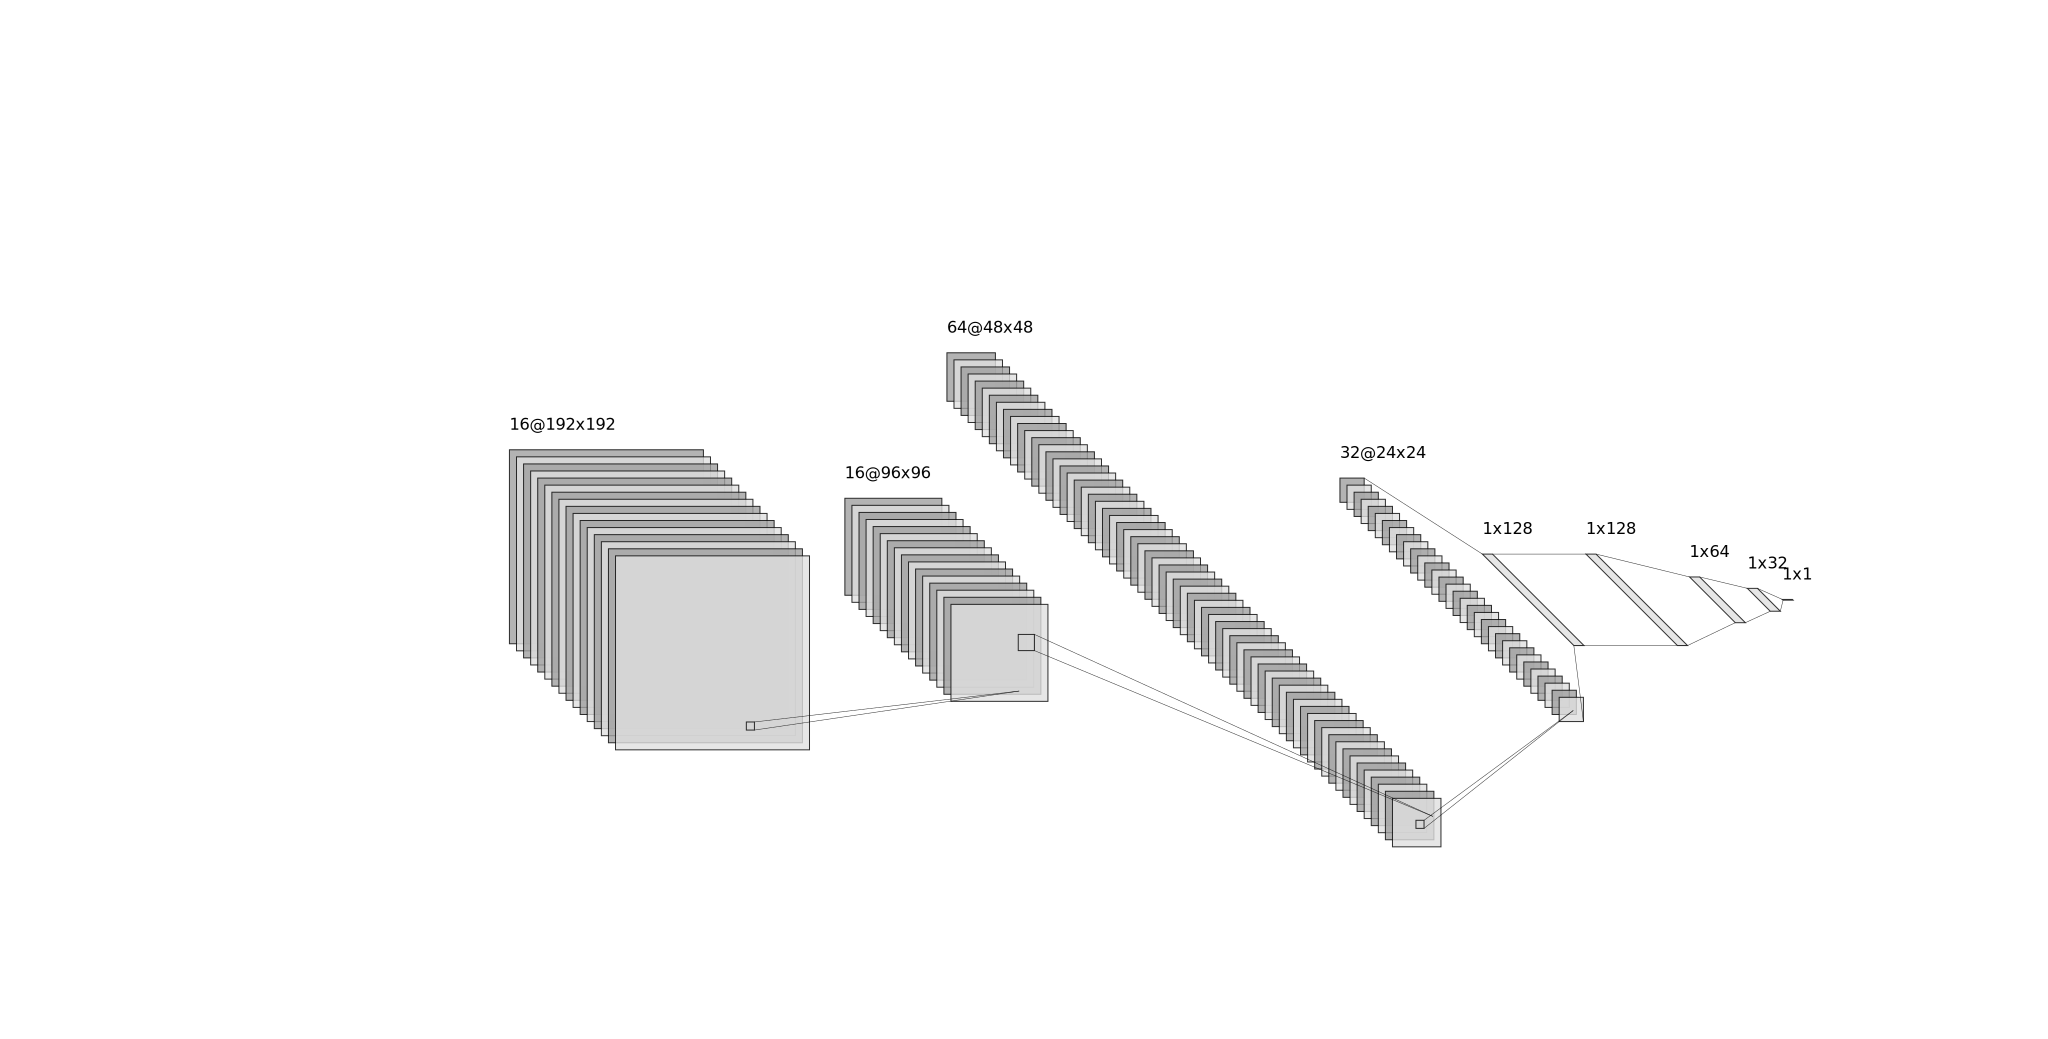
\includegraphics[width=\textwidth]{img/nn}
	\end{center}
\end{frame}

\begin{frame}{Last Bit of Scenario, I Promise}
	We use:
	\begin{enumerate}[label=\alph*.]
		\item Optimizer: \texttt{Adam}
			\begin{enumerate}[label=-]
				\item Learning Rate: $10^{-2}$
				\item Epsilon: $10^{-8}$
			\end{enumerate}
		\item Loss: \texttt{BinaryCrossEntropy}
	\end{enumerate} \pause
	After training, we achieve a test accuracy of \texttt{0.5000}. This \textit{sucks}. \pause \newline \\

	Here are some misclassified samples:
	\begin{center}
		\hspace*{-7em}
		\includegraphics[width=10cm]{img/misclassifications}
	\end{center}

	\vspace{-1em}
	How can we diagnose the cause of this?
\end{frame}

\section{Baselining Interpretability}

\begin{frame}{What even \textit{is} Interpretability?}
	\begin{columns}
		\begin{column}{0.5\textwidth}
			\begin{center}
				\includegraphics[width=5cm]{img/1838} \pause
			\end{center}
		\end{column}
		\begin{column}{0.5\textwidth}
			Interpretability within Machine Learning is the \textbf{degree} to which we can understand the \textbf{cause} of a decision, and use it to consistently \underline{predict the model's prediction}. \pause \newline \\

			This is easy for shallow learning. \pause For deep learning however, it is a \textbf{lot harder}.
		\end{column}
	\end{columns}
\end{frame}

\begin{frame}{A Cautionary Tale}
	\begin{columns}
		\begin{column}{.6\textwidth}
			\begin{figure}
				\hspace*{.5em}
				\includegraphics[width=.98\textwidth]{img/bias}
				\vspace{-1.5em}
				\centering
				\caption*{\footnotesize \ \ \ \ \ \url{https://interaktiv.br.de/ki-bewerbung/en/}}
			\end{figure}
		\end{column}
		\begin{column}{.03\textwidth}
		\end{column}
		\begin{column}{.4\textwidth}
			Start-up attempting to make the application process `faster, but also more objective and fair'. \pause \newline \\
			They were not successful.
		\end{column}
	\end{columns}
\end{frame}

\begin{frame}{Class Activation Mappings}
	For deep learning, interpretability techniques today involve a fairly straightforward formula: \pause
	\begin{enumerate}[label=-]
		\item Split hidden layers.
		\item Expose weights.
		\item \textit{Observe!} \pause
	\end{enumerate}
	We'll focus today's discussion on \textbf{Class Activation Mappings (CAMs)}:
	\vspace{1em} \includegraphics[width=9.5cm]{img/cams}
\end{frame}

\begin{frame}{Building Feedback Loops}
	Finding optimal model weights is an \textbf{NP-hard} problem. \pause \\
	\begin{columns}
		\begin{column}{.5\textwidth}
			\begin{figure}
				\includegraphics[width=4.5cm]{img/np}
				\caption*{\footnotesize Model Search Space}
			\end{figure} \pause
		\end{column}
		\begin{column}{.5\textwidth}
			We can't speed this up. However, we do have information about our training set that we can use to \textbf{motivate training behaviour}. \pause \newline \\
		\end{column}
	\end{columns}
	So, the idea here is simple: use \underline{shared knowledge} (+ common sense) to modify how we train our models.
\end{frame}

\section{Leveraging Interpretability}
\begin{frame}{Getting Back to the Challenge}
	There are some obvious causes for why it performs poorly:
	\begin{enumerate}[label=\alph*.]
		\item There are too few, unbalanced training samples. \pause \\
			\underline{Solution:} Data Augmentation \pause
		\item \textbf{The images have a sharp color dominance.} \pause
			\begin{center}
				\vspace{-1em}
				\hspace*{-2em}  
				\includegraphics[width=\textwidth]{img/dataset.pdf}
			\end{center}
	\end{enumerate}
\end{frame}

\begin{frame}{Diagnosing the Model}
	When we obtain a Class Activation Map of a sample image, we observe:
	\begin{center}
		\vspace{-.8em}
		\includegraphics[width=8cm]{img/bad-cam}
	\end{center} \pause
	\vspace{-1em}
	It \textbf{does not} use the leopard to base it's prediction!
	This is prevalent \underline{across the dataset}. \pause \newline \\

	\textbf{Observation:} The targets in our entire training dataset are centered. \pause \newline \\

	Q: Can we exploit this?
\end{frame}

\begin{frame}{Introducing \texttt{CAMLoss}!}
	Here's the idea:
	\begin{enumerate}[label=\alph*.]
		\item In addition to the prediction, we output the class activation map. \pause
		\item We extract a random subset of the \textbf{top portion} of the map. \pause
		\item We return the mean of the weights. Weights $\propto \frac{1}{\text{Fit Quality}}$ \pause
		\item This is our additional self-supervised loss function! \pause
	\end{enumerate}
	Obtaining the Class Activation Map of the updated model, we observe:
	\begin{center}
		\vspace{-.9em}
		\includegraphics[width=10cm]{img/fixed-cam}
	\end{center} \pause
	\vspace{-1em}
	\textbf{Great Success!}
\end{frame}

\begin{frame}{Thank you!}
	\begin{center}
		Have an awesome rest of your day! Any questions for me?
	\end{center}
	\begin{center}
		\textbf{Code, Experiments, Data, Slides:} \url{https://dagshub.com/jinensetpal/tmls22.git}
	\end{center}
\end{frame}

\end{document}
